\subsection{Contratiempos}

Sin embargo, este proceso de diseño y fabricación de PCB no fue sin sus contratiempos y errores, que hubieron de ser resueltos previamente a poder realizar pruebas y ensayos con la placa. Estos inconvenientes fueron dados por falta de experiencia en el ámbito de diseño de PCB y utilización de software EDA, en especial para el diseño de una placa tan compleja.\\

Muchos de estos errores fueron detectados previamente al proceso de fabricación y pudieron ser corregidos en el esquemático de PCB dentro de KiCad. Por ejemplo, en el diseño inicial del circuito para las ondas PWM de los transistores, se habían utilizado los puertos de ePWM incorrectos que hubiesen dificultado la implementación del control de ciclo de trabajo mediante phase-shift, pero en una revisión de los archivos de diseño previo a la fabricación se encontró y rectificó este error.\\

\subsubsection{Footprint de MOSFET}

SEl error de diseño más importante en la placa se descubrió una vez que ya habían arribado las placas impresas al laboratorio. Durante las fases tempranas del diseño de la placa se colocaron las cuatro footprints TO-247 correspondientes a los MOSFET IRFP150, pero por desconocimiento, se elaboró su footprint en base a la modificación de otra, en vez de obtenerla de las bibliotecas online ya mencionadas.\\

La footprint para estos transistores que se encuentra sobre la placa tiene sus terminales colocados en el orden \textit{Drain-Gate-Source}. Sin embargo, el IRFP150 y todos los MOSFET de potencia de paquete TO-247 tienen el terminal Gate en la primera posición, con el orden \textit{Gate-Drain-Source}.\\

\paragraph{Placa Adaptadora}

Se evaluaron varias soluciones para este problema, incluso buscando modelos alternativos de MOSFET de potencia que tuvieran los terminales en el orden necesario. La solución por la que se optó fue diseñar una pequeña placa adaptadora simple faz que se conecte en la posición original de los transistores, y con las pistas de cobre invertir la posición de lo terminales de drain y gate.\\

\begin{figure}[h]
    \centering
    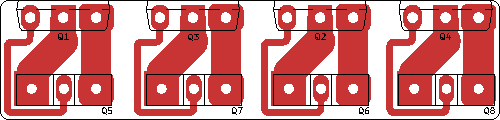
\includegraphics[scale=1.2]{Imagenes/Placa Adaptadora.pdf}
    \caption{Diagrama de la capa de cobre de la placa adaptadora diseñada para mitigar el error de diseño.}
    \label{placa_adaptadora}
\end{figure}

En su diseño se tuvo que buscar hacer la placa lo más pequeña posible, ya que los transistores tienen borneras y otros componentes alrededor que limitan cuan grande puede ser. Además, la nueva fooprint de los MOSFET debía quedar lo más cercana posible al borde de la placa, para facilitar el montaje del disipador de los transistores.\\

Una vez que se finalizó el diseño, que no llevó más de un par de días, se utilizaron las instalaciones disponibles en el ATEI (Área Técnica de Electrónica e Instrumental), y con una placa de cobre simple faz, se fabricó la placa adaptadora que luego se soldó por sobre la placa original.\\